\documentclass[11pt,journal]{IEEEtran}
\usepackage{lipsum}
\usepackage[T1]{fontenc}
\usepackage{fouriernc}
\usepackage{cases}
\usepackage{amsmath}
\usepackage[noadjust]{cite}
\usepackage{hyperref}
\usepackage{multirow}
\usepackage{graphicx}
\usepackage{adjustbox}
\usepackage{makecell}
\usepackage[dvipsnames]{xcolor}
\usepackage{tikz}



\hypersetup{
    colorlinks=true,
    linkcolor=blue,
    anchorcolor=blue,
    urlcolor=blue,
    citecolor=blue
}
\graphicspath{ {./imgs/} }
\newcommand{\eq}{\; = \;}
\newcommand{\nl}{

\medskip

}

\title{FIRE CLASSIFICATION WITH A DEEP LEARNING APPROACH}
\author{Davide Avolio \quad Francesca Cinelli}

\begin{document}

\maketitle

\begin{abstract}
As a challenge, we were asked to perform a binary classification of images, to identify the ones with fire and the ones without fire.
\end{abstract}

\begin{IEEEkeywords}
    DEEP LEARNING, \\
    COMPUTER VISION, VISUAL TRANSFORMER,\\
    CNN, IMAGE CLASSIFICATION, FIRE
\end{IEEEkeywords}

\section{Dataset and preprocessing}
The dataset provided is composed of 15.609 images, split in train, validation and test set. All the images are 224×224 and the test set ones are unlabeled. \nl
after analyzing the dataset, the following images were moved from the folder of class 1 to the folder of class 0: 15196, 6510, 7991, 10269, 11602, 12441, 14595, 6173, 6900 (from the train set folder) and 6631 (from the validation set folder). \nl
By looking at the images classified as "fire", we noticed that most of them contain flames, while another remarkable part has smoke and a smaller set is with firefighters. We decided to split the training set in three classes:
\begin{itemize}
	\item class 0: images that are neither fire nor smoke
	\item class 1: images with smoke
	\item class 2: images with fire
\end{itemize}
To perform this division, we built another program, the "Fire Smoke Divider"\cite{firesmokedivider} that works in this way: given the folder containing all the fire images, it does a color classification and divides the images based on the amount of red and yellow pixels in them. The program works with the library OpenCV. After running the program we then refined this further classification manually. \nl
After this classification, we decided to train the model on these three classes and then merging them into two, but we didn't get an important improvement, so we switched back to the original two.

\section{Models from scratch}
The first approach to the problem was to implement from scratch a model, see its performance and then pass to a more complex one. \nl
The first model we used was a simple MLP\cite{MLP}, with two linear layers and ReLU and a final layer with two neurons to output the result. After the training, we got a Train Accuracy of 72.88\% and a Validation Accuracy of 75.13\%.\nl
The second model we used was a simple CNN\cite{CNN}, with three Convolutional layers, ReLU and Max Pool and final two linear layers for the output. After the training, we got a Train Accuracy of 87.63\% and a Validation Accuracy of 88.33\%, an improvement with respect to the MLP. \nl

\section{Densenet}
After the simple CNN, we decided to use a pretrained model, Densenet. The idea behind Densenet is the use of Dense blocks, convlutional layers that are all connected to each other; moreover, each layer obtains additional inputs from all the preceding layers, so to maintain the feed-forward structure.
The best values were obtained in the second epoch (Train Loss: 0.1787, Val Loss: 0.0603, Val Accuracy: 0.9833)

\begin{figure}[ht]
	\renewcommand{\arraystretch}{2.0}
	\label{DenseNet_TrainVal_Loss}
	\centering
	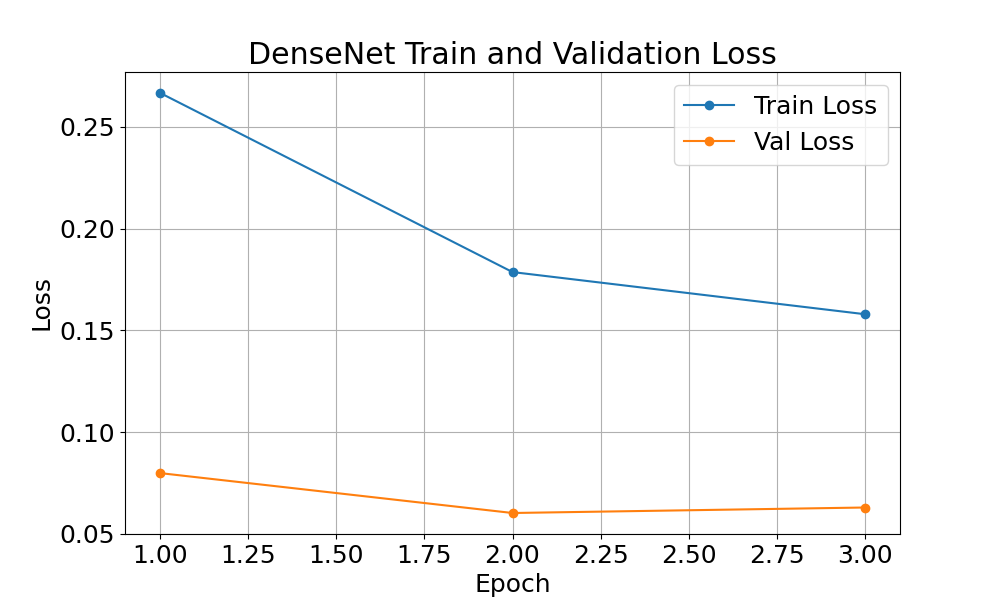
\includegraphics[width=\linewidth]{DenseNet_TrainVal_Loss}
	\caption{Train and Validation loss obtained with the DenseNet model}
\end{figure}

\begin{figure}[ht]
	\renewcommand{\arraystretch}{2.0}
	\label{DenseNet_Val_Accuracy}
	\centering
	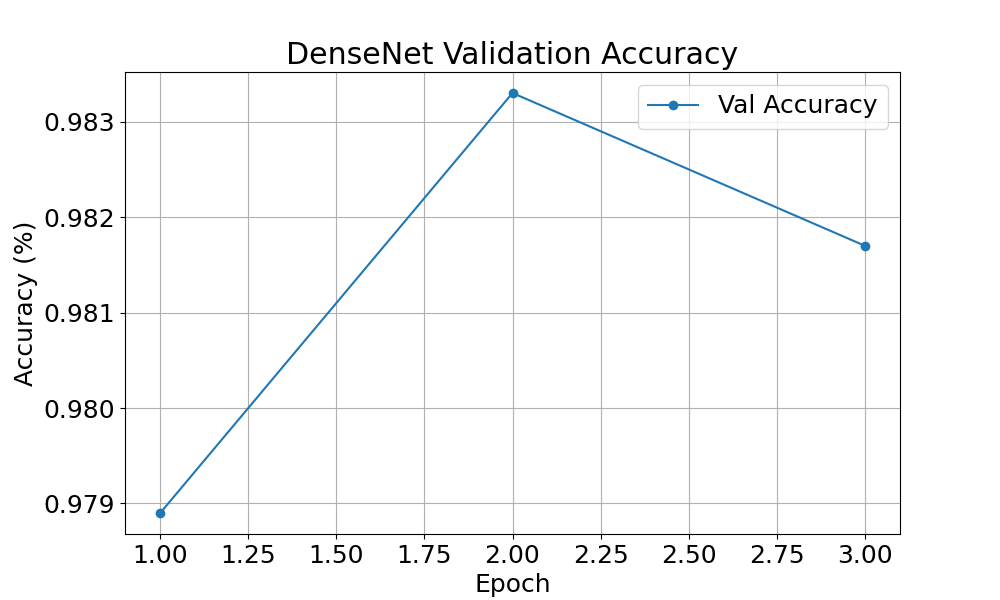
\includegraphics[width=\linewidth]{DenseNet_Val_Accuracy}
	\caption{Validation accuracy obtained with the DenseNet model}
\end{figure}
\section{ViT}
The last model we tried is the Vision Transformer (ViT)\cite{ViT}. This model exploits a different architecture rather than the Densenet: as the name suggests the main component is the transformer. Each image is divided in a patch (in our case 16×16 patches) that are then embedded into vectors and processed by the encoder.
Given the considerations about the training set, we decided to modify this architecture and add another linear layer before the output one. This new layer has 3 neurons, one for each subclass, that are conveyed to the output layer with 2 neurons.
We performed again the training and we obtained better results than the Densenet:
\begin{figure}[ht]
	\renewcommand{\arraystretch}{2.0}
	\label{VitModel_TrainVal_Loss}
	\centering
	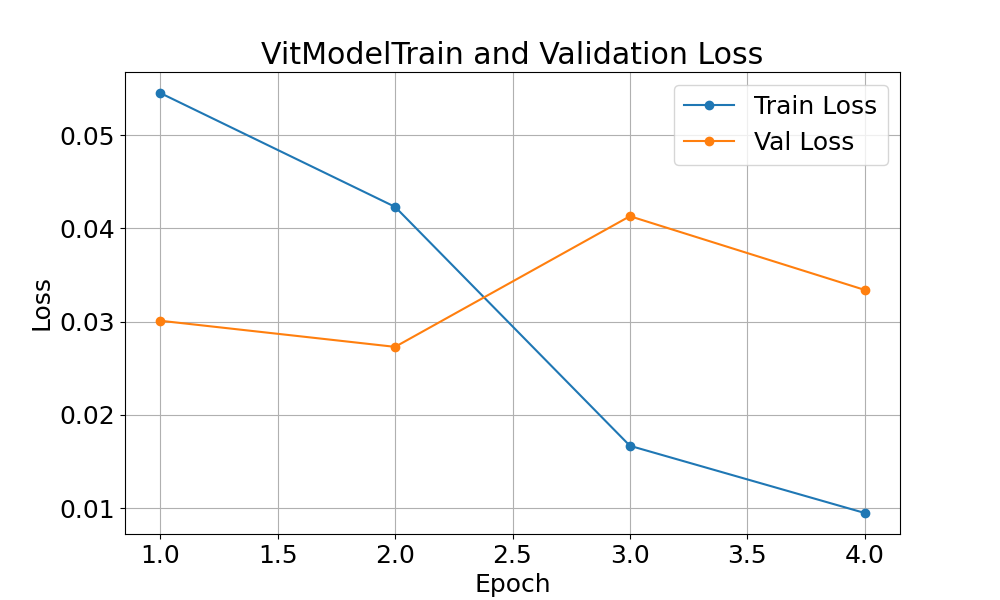
\includegraphics[width=\linewidth]{VitModel_TrainVal_Loss}
	\caption{Train and Validation loss obtained with the ViT model}
\end{figure}

\begin{figure}[ht]
	\renewcommand{\arraystretch}{2.0}
	\label{VitModel_Val_Accuracy}
	\centering
	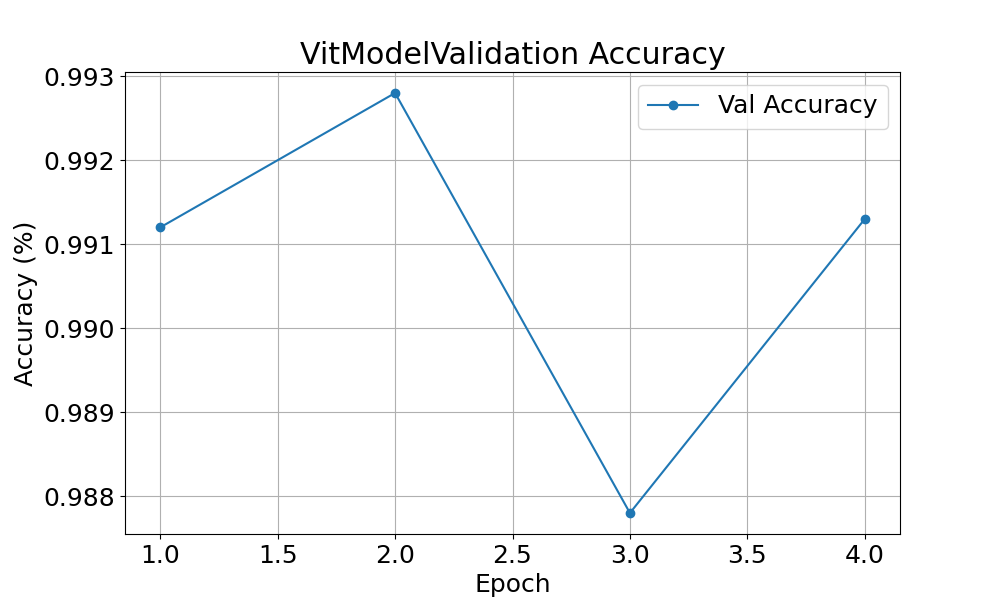
\includegraphics[width=\linewidth]{VitModel_Val_Accuracy}
	\caption{Validation accuracy obtained with the ViT model}
\end{figure}
In particular, the second epoch gave the best results and after that the model went overfitting.
\section{Conclusion}
As we can see from the series of models used, by analyzing the structure of the dataset, it was possible to obtain a better performance. In the simplest model, the MLP, we weren't making any assumption on the data, but we were simply using full connections between layers, while in the others there were more complex layers, modified in such a way to study better the data.
Finally, we saw the difference between a normal model and a pretrained one, with this second kind performing much better. This difference is given by the fact that the images classified as fire are not only images of flames, but spread on a wider range of entities and shapes (flames, smoke, firefighters, Canadair, Firetrucks, ash), some of which can be correctly identified only after a training on multiple images. This can help for example by spotting the differences between a firefighter and a normal person or a Canadair with a normal plane and this is what can make the model perform at its best.


\begin{thebibliography}{9}
	\bibitem{firesmokedivider}
	\url{https://github.com/slashm4n/Fire-Classifier/blob/master/Models/FireSmokeDivider.py}
	\bibitem{MLP}
	\url{https://github.com/slashm4n/Fire-Classifier/blob/master/Models/MLP.py}
	\bibitem{CNN}
	\url{https://github.com/slashm4n/Fire-Classifier/blob/master/Models/CNN.py}
	\bibitem{ViT}
	\url{https://github.com/slashm4n/Fire-Classifier/blob/master/Models/Vit.py}
\end{thebibliography}
\end{document}